\documentclass[12pt,runningheads]{llncs}
% ── Packages ──────────────────────────────────────────────────────────────────
\usepackage[T1]{fontenc}
\usepackage{graphicx}
\usepackage{amsmath}
\usepackage{amssymb}
\usepackage{tabularx}
\usepackage{array}
\usepackage{booktabs}
\usepackage{float}
\usepackage{xcolor}
% \usepackage{times}
% \usepackage{setspace}
% \usepackage{titlesec}
% \usepackage{amsmath}
% \usepackage{amssymb}
% \usepackage[table]{xcolor}
% \usepackage{hyperref}
% \usepackage{microtype}
% \usepackage{enumitem}
% \usepackage{fancyhdr}
% \usepackage{indentfirst}
% \usepackage{parskip}
% \usepackage[numbers]{natbib}

\newcolumntype{L}[1]{>{\raggedright\arraybackslash}p{#1}}
\newcolumntype{C}[1]{>{\centering\arraybackslash}p{#1}}

\begin{document}

\title{An Experimental Analysis of Machine Learning Project for American Sign Language}

\titlerunning{ML Models for ASL Recognition}

\author{
Kate D. Capadocia \and
Gabriel Dominic A. Dicar \and
Earl Sheldon F. Pabua \and
Ara Abigail E. Ambita
}
\authorrunning{Capadocia et al.}

\institute{
Department of Physical Sciences and Mathematics\\
University of the Philippines Visayas, Miagao, Iloilo, Philippines
}

\maketitle

% \begin{abstract}
% This study investigates the performance of classical machine learning algorithms for American Sign Language (ASL) alphabet recognition using image-based data. Support Vector Machine (SVM), k-Nearest Neighbors (k-NN), Naïve Bayes, and Random Forest classifiers are evaluated under identical experimental conditions to determine their effectiveness in recognizing static ASL hand gestures. The study aims to identify lightweight and computationally efficient alternatives to deep learning approaches for resource-constrained environments.

% \keywords{American Sign Language \and Machine Learning \and Gesture Recognition \and Computer Vision}
% \end{abstract}

\section{Introduction}

Communication is a fundamental human need that enables individuals to convey information, express emotions, and participate meaningfully in social and professional life. According to the World Health Organization \cite{who2021}, approximately 1.57 billion people worldwide live with some degree of hearing loss, a figure projected to rise to 2.5 billion by 2050. For this population, verbal communication is frequently inaccessible, making alternative modalities essential. American Sign Language (ASL) serves as the primary language of the Deaf and hard-of-hearing communities in the United States and Canada. As a complete, natural language with its own grammar, syntax, and expressive conventions, ASL conveys meaning through the coordinated movement of the fingers, hands, arms, and body, supplemented by facial expressions \cite{bakershenk1980}.

Despite its linguistic richness and the size of the community that depends on it, ASL is not widely known among hearing individuals. This asymmetry creates a persistent communication barrier that contributes to the social, educational, and occupational marginalization of the Deaf community. Interpreter services, while valuable, are costly and not always available in real-time or informal settings. Automated sign language recognition (SLR) systems present a promising technological solution: by translating hand gestures into readable text, such systems can act as always-available communication bridges that reduce dependence on human interpreters and promote greater social inclusivity.

% ══════════════════════════════════════════════════════════════════════════════
\subsection{Review of Related Literature}

Research in automated sign language recognition has followed two broad hardware paradigms: sensor-based and vision-based approaches. Sensor-based systems employ wearable devices such as data gloves equipped with flex sensors, accelerometers, and Inertial Measurement Units (IMUs), to directly measure hand joint angles and spatial orientation. While these devices can yield high recognition accuracy, their reliance on specialized hardware constrains natural interaction and limits practical accessibility for everyday use \cite{oz2011}.

Vision-based approaches offer a non-intrusive alternative by extracting hand features from standard RGB camera images. Within this paradigm, classical machine learning algorithms have been widely studied for static sign recognition. Support Vector Machines (SVMs) have proven particularly effective due to their ability to find optimal decision boundaries in high-dimensional feature spaces. \cite{barczak2011} demonstrated that an SVM operating on normalized hand-shape descriptors could reliably classify static ASL letters, while \cite{isaacs2004} similarly applied SVMs to fingerspelling recognition with favorable results. The flexibility of SVMs in handling non-linearly separable data through kernel functions particularly the Radial Basis Function (RBF) kernel that makes them well-suited to the complex geometric variation inherent in hand gesture data.

Random Forest classifiers, as ensemble methods that aggregate predictions from multiple decision trees trained on random feature subsets, have also attracted considerable interest for gesture recognition tasks due to their robustness to noise and resistance to overfitting. \cite{pugeault2011} employed a Random Forest on depth-image features for finger-spelling recognition, achieving strong multi-class performance. The model's ability to rank feature importances provides an additional analytical benefit, enabling researchers to identify which landmark positions contribute most to discriminating between visually similar signs.

The k-Nearest Neighbors (k-NN) algorithm, though simple in formulation, has served as a consistent baseline in sign language recognition studies. Its non-parametric nature requires no explicit model training, and it performs well when the feature space is compact and class clusters are well-separated. \cite{hasan2012} demonstrated competitive k-NN performance on hand gesture feature vectors, noting that the choice of distance metric and the number of neighbors $k$ are the primary factors governing classification quality. The introduction of standardized feature scaling further amplifies k-NN effectiveness by ensuring that no single dimension dominates the distance computation.

Gaussian Na\"{i}ve Bayes (GNB) represents a probabilistic baseline frequently included in comparative gesture recognition studies. By modeling each feature as an independent Gaussian distribution per class, GNB is computationally efficient and requires minimal data to estimate parameters. While its conditional independence assumption is known to be violated in structured hand pose data where landmark coordinates exhibit strong spatial correlations, the classifier nonetheless provides useful performance context against which more expressive models can be measured \cite{rish2001}.

A key advancement enabling more effective classical ML classification of hand gestures was the release of MediaPipe Hands by Google \cite{zhang2020}. This real-time hand landmark detection framework estimates 21 three-dimensional keypoints from a single RGB frame, producing a structured skeletal representation of the hand. By reducing raw images to a 63-dimensional coordinate vector $\mathbf{f} \in \mathbb{R}^{63}$, MediaPipe Hands abstracts away appearance-level variation, including skin tone, background clutter, and illumination differences, while preserving the geometric configuration that distinguishes one sign from another. Recent studies have confirmed that classical ML classifiers operating on such landmark-based features can achieve high accuracy on static gesture datasets, with the additional advantage of being computationally lightweight and deployable without GPU hardware \cite{adeyanju2021,bantupalli2018}.

% ══════════════════════════════════════════════════════════════════════════════
\subsection{Problem Statement}

While individual classical ML classifiers have been applied to sign language recognition in prior work \cite{barczak2011,pugeault2011,hasan2012}, a systematic and reproducible comparison of multiple algorithms (SVM, k-NN, Gaussian Na\"{i}ve Bayes, and Random Forest) under a unified experimental framework on MediaPipe hand landmark features has not been thoroughly established for the full 26-class ASL static alphabet. Existing studies vary in their datasets, preprocessing pipelines, feature representations, and evaluation protocols, making direct performance comparisons unreliable. Without a controlled benchmark, practitioners have limited guidance on which classifier offers the best trade-off between recognition accuracy, generalization stability, and computational efficiency for a hardware-free, vision-based ASL alphabet recognition system.

% ══════════════════════════════════════════════════════════════════════════════
\subsection{Objectives of the Study}

This study addresses the identified gap through the following specific objectives:

\begin{enumerate}
  \item To construct a structured feature dataset by extracting 63-dimensional hand landmark coordinate vectors from the ASL Alphabet image set using the MediaPipe Hands framework \cite{zhang2020}.

  \item To train and evaluate four classical machine learning classifiers such as Support Vector Machine (SVM), k-Nearest Neighbors (k-NN), Gaussian Na\"{i}ve Bayes, and Random Forest on the extracted landmark features for the recognition of all 26 letters of the ASL static alphabet.

  \item To assess each classifier using a consistent evaluation protocol comprising a stratified 80/20 holdout split and 5-fold stratified cross-validation, reporting accuracy, weighted precision, recall, F1-score, and cross-validation mean accuracy.

  \item To identify the classifier that achieves the optimal balance between recognition accuracy and generalization stability for deployment in a lightweight, hardware-free ASL alphabet recognition system.
\end{enumerate}

% ══════════════════════════════════════════════════════════════════════════════
\subsection{Hypotheses}

Based on the reviewed literature and the chosen methodology, this study proposes the following hypotheses:

\textbf{H\textsubscript{1}} The 63-dimensional hand landmark features extracted using MediaPipe Hands \cite{zhang2020} are sufficient for accurate recognition of the 26 ASL alphabet classes.

\textbf{H\textsubscript{2}} The SVM with RBF kernel is expected to achieve the highest classification accuracy among the evaluated models \cite{barczak2011,isaacs2004}.

\textbf{H\textsubscript{3}} Random Forest is expected to produce the most stable performance across cross-validation folds due to its ensemble-based structure \cite{pugeault2011}.

\textbf{H\textsubscript{4}} Gaussian Na\"{i}ve Bayes is expected to achieve the lowest overall accuracy because of its independence assumption on correlated hand landmark features \cite{rish2001}.
% ══════════════════════════════════════════════════════════════════════════════
\section{Scope and Limitations}

This study is limited to the recognition of the 26 static hand configurations corresponding to the letters A through Z of the American Sign Language alphabet. Dynamic gestures, ASL words, phrases, or sequences involving hand motion over time are outside the scope of this work. The pipeline operates entirely on still images drawn from the ASL Alphabet dataset, and classification is performed on an image-by-image basis rather than on continuous video streams. The study does not conduct signer-independent evaluation across external datasets; generalization performance is estimated through stratified cross-validation on the single dataset used for training \cite{adeyanju2021}. These boundaries allow for a focused and reproducible comparison of the four selected classical ML classifiers under controlled and consistent experimental conditions.

% ══════════════════════════════════════════════════════════════════════════════
\section{Significance of the Study}

This study contributes to the broader effort of making communication technology more inclusive and accessible for the Deaf and hard-of-hearing communities \cite{who2021,bakershenk1980}. By establishing a rigorous benchmark of four classical machine learning classifiers on MediaPipe hand landmark features \cite{zhang2020} for the full 26-class ASL alphabet, this work provides a transparent, reproducible, and computationally lightweight reference point for future research. The findings offer practical guidance for developers building real-time ASL recognition applications on consumer-grade hardware without the need for GPU acceleration or large-scale infrastructure, lowering the barrier to entry for assistive technology development in resource-constrained environments \cite{adeyanju2021,bantupalli2018}.

\section{Methodology}
% ─────────────────────────────────────────────────────────────────────────────

This study follows a two-stage machine learning pipeline consisting of (1) data processing and feature extraction, and (2) model training and evaluation. Raw ASL alphabet images are first transformed into structured numerical representations using hand landmark detection. These features are then used to train and evaluate multiple classification models to determine the best-performing algorithm for ASL recognition.

% ─────────────────────────────────────────────────────────────────────────────
\subsection{Dataset}
The dataset used in this study consists of 26 classes corresponding to the ASL alphabet letters A to Z. Each class contains 3000 labeled images of static hand gestures captured in RGB format. The dataset is organized into separate directories per class, where each directory represents one ASL letter.

\begin{figure}[H]
\centering

\begin{tabular}{ccccc}

\includegraphics[width=0.18\textwidth]{sample_a.jpg} &

\includegraphics[width=0.18\textwidth]{sample_b.jpg} &

\includegraphics[width=0.18\textwidth]{sample_c.jpg} &

\includegraphics[width=0.18\textwidth]{sample_d.jpg} &

\includegraphics[width=0.18\textwidth]{sample_e.jpg} \\

(a) A &
(b) B &
(c) C &
(d) D &
(e) E \\
\end{tabular}

\caption{Sample ASL Hand Gesture Images from the Dataset}
\label{fig:asl_samples}

\end{figure}
Figure~\ref{fig:asl_samples} shows sample images from the ASL dataset used in the study. Each image is treated as an independent sample and is processed individually through the feature extraction pipeline. The dataset is traversed systematically by iterating through all class folders for preprocessing and landmark extraction.

\subsection{Image Preprocessing}
Before feature extraction, each image undergoes a standardized preprocessing pipeline to ensure consistency and improve detection reliability.

\subsubsection{Spatial Normalization}
All images are resized to a fixed resolution of $512 \times 512$ pixels using bilinear interpolation. This ensures uniform input dimensions regardless of the original image size and aspect ratio.

\subsubsection{Noise Reduction}
A Gaussian blur filter with a $3 \times 3$ kernel ($\sigma = 0$) is applied to reduce high-frequency noise while preserving essential structural features of the hand.

\subsubsection{Contrast Enhancement}
Image contrast and brightness are adjusted using a linear transformation:

\[
I' = \alpha I + \beta
\]

where $\alpha = 1.2$ (contrast factor) and $\beta = 15$ (brightness offset). This enhances the visibility of hand regions against varying backgrounds.

\subsubsection{Color Space Conversion}
Since OpenCV loads images in BGR format, each image is converted to RGB using \texttt{cv2.cvtColor} to ensure compatibility with MediaPipe Hands.

% ─────────────────────────────────────────────────────────────────────────────
\subsection{Hand Landmark Detection}

Hand landmark detection is performed using MediaPipe Hands, a real-time hand tracking framework developed by Google. The system operates in static image mode and is configured to detect a single hand per image.

MediaPipe Hands uses a two-stage pipeline:

\begin{itemize}
\item A palm detection model that identifies the region of interest.
\item A landmark model that predicts 21 hand keypoints.
\end{itemize}

Each successful detection returns 21 landmarks corresponding to anatomical points of the hand, including the wrist, finger joints, and fingertips. Each landmark contains $(x, y, z)$ coordinates normalized relative to the image.

Images where no hand is detected are excluded from the final dataset.

% ─────────────────────────────────────────────────────────────────────────────
\subsection{Feature Vector Construction}

Each of the 21 detected hand landmarks is associated with a three-dimensional coordinate tuple $(x, y, z)$, where $x$ and $y$ are normalized to the image width and height respectively (range $[0, 1]$), and $z$ represents the estimated depth relative to the wrist landmark. Concatenating the coordinates across all 21 landmarks yields a 63-dimensional feature vector:

\begin{equation}
  \mathbf{f} = \bigl[x_0,\, y_0,\, z_0,\; x_1,\, y_1,\, z_1,\; \ldots,\; x_{20},\, y_{20},\, z_{20}\bigr] \in \mathbb{R}^{63}
\end{equation}

This representation encodes the spatial configuration of the entire hand skeleton in a compact, pose-based descriptor that is invariant to non-informative low-level visual variations such as skin tone, lighting conditions, and background texture, properties that raw pixel-based features do not inherently provide.

\begin{table}[htbp]
\centering
\caption{Mapping of Hand Landmark Indices to Anatomical Regions}
\label{tab:landmarks}
\renewcommand{\arraystretch}{1.25}

\begin{tabularx}{\linewidth}{C{3cm} C{4cm} L{6cm}}
\hline
\textbf{Landmark Index} & \textbf{Feature Components} & \textbf{Description} \\
\hline

0 & $(x_0,y_0,z_0)$ & Wrist \\

1--4 & $(x_1,y_1,z_1)$ to $(x_4,y_4,z_4)$ & Thumb (CMC to Tip) \\

5--8 & $(x_5,y_5,z_5)$ to $(x_8,y_8,z_8)$ & Index Finger (MCP to Tip) \\

9--12 & $(x_9,y_9,z_9)$ to $(x_{12},y_{12},z_{12})$ & Middle Finger (MCP to Tip) \\

13--16 & $(x_{13},y_{13},z_{13})$ to $(x_{16},y_{16},z_{16})$ & Ring Finger (MCP to Tip) \\

17--20 & $(x_{17},y_{17},z_{17})$ to $(x_{20},y_{20},z_{20})$ & Pinky Finger (MCP to Tip) \\

\hline
\end{tabularx}
\end{table}

% ─────────────────────────────────────────────────────────────────────────────
\subsubsection{Dataset Construction}

All extracted feature vectors are aggregated into a structured dataset stored in CSV format. The dataset consists of 63 numerical feature columns and one label column representing the corresponding ASL class.

The final dataset is represented as:

\[
\mathbf{X} \in \mathbb{R}^{N \times 63}, \quad \mathbf{y} \in \mathbb{R}^{N}
\]

where $N$ is the total number of successfully processed images.

Each feature column corresponds to a specific landmark coordinate (e.g., $x_0, y_0, z_0, \dots, x_{20}, y_{20}, z_{20}$).

% ─────────────────────────────────────────────────────────────────────────────
\subsection{Data Preparation for Modeling}

\subsubsection{Label Encoding}

Since the target labels are categorical (A–Z), they are converted into numerical form using label encoding. Each ASL letter is mapped to a unique integer value to allow compatibility with machine learning algorithms.

\subsubsection{Train-Test Split}

The dataset is divided into training (80\%) and testing (20\%) sets using stratified sampling. Stratification ensures that all 26 classes are proportionally represented in both subsets, preserving the original class distribution.

\subsubsection{Feature Scaling}

Feature standardization is applied using z-score normalization:

\[
x' = \frac{x - \mu}{\sigma}
\]

where $\mu$ is the mean and $\sigma$ is the standard deviation computed from the training set only. This prevents data leakage and ensures consistent scaling across models.


% ══════════════════════════════════════════════════════════════════════════════
\subsection{Machine Learning Models}

Four classical machine learning models are evaluated under identical conditions:

\subsubsection{Support Vector Machine (SVM)}

A Support Vector Machine with Radial Basis Function (RBF) kernel is used to handle non-linear decision boundaries. The RBF kernel is defined as:

\[
K(\mathbf{x}_i, \mathbf{x}_j) = \exp(-\gamma \|\mathbf{x}_i - \mathbf{x}_j\|^2)
\]

where $\gamma$ controls the influence of individual training samples.

\subsubsection{k-Nearest Neighbors (k-NN)}

The k-NN classifier uses $k = 5$ neighbors and Euclidean distance to classify samples based on majority voting among nearest points in feature space.

\subsubsection{Gaussian Naïve Bayes}

Gaussian Naïve Bayes assumes feature independence and models each feature using a Gaussian distribution. Classification is performed using Bayes’ theorem:

\[
P(y \mid \mathbf{x}) \propto P(y) \prod_{j=1}^{63} P(x_j \mid y)
\]

\subsubsection{Random Forest}

Random Forest is an ensemble learning method consisting of 100 decision trees. Each tree is trained on a bootstrap sample, and at each split, a subset of features is randomly selected. Final predictions are obtained through majority voting.

\begin{table}[htbp]
\centering
\caption{Machine Learning Model Configurations}
\label{tab:models}
\renewcommand{\arraystretch}{1.2}

\begin{tabularx}{\linewidth}{L{3cm} L{3cm} L{6.3cm}}
\hline
\textbf{Model} & \textbf{Type} & \textbf{Key Hyperparameters} \\
\hline

SVM & Kernel-based & RBF kernel, $C = 1.0$, $\gamma = \text{scale}$ \\

k-NN & Instance-based & $k = 5$, Euclidean distance \\

Gaussian Naïve Bayes & Probabilistic & Gaussian likelihood, uniform priors \\

Random Forest & Ensemble & 100 trees, max features $\sqrt{p}$, random state 42 \\

\hline
\end{tabularx}
\end{table}

% ══════════════════════════════════════════════════════════════════════════════
\subsection{Model Evaluation}

\subsubsection{Data Splitting}

Models are evaluated using an 80/20 train-test split. Performance metrics are computed on the unseen test set to assess generalization capability.

\subsubsection{Cross-Validation}

A 5-fold stratified cross-validation approach is used to evaluate model stability. The dataset is divided into 5 folds, and each fold is used once as validation data while the remaining folds are used for training.

The final score is reported as the mean accuracy across all folds.

% ══════════════════════════════════════════════════════════════════════════════
\subsection{Evaluation Metrics}

Model performance is measured using the following metrics:

\begin{itemize}
\item \textbf{Accuracy:} Overall correctness of predictions
\item \textbf{Precision:} Correct positive predictions over total predicted positives
\item \textbf{Recall:} Correct positives over actual positives
\item \textbf{F1-score:} Harmonic mean of precision and recall
\end{itemize}

All metrics are computed using weighted averaging to account for class distribution imbalance.
\section{Results and Discussion}

This chapter presents the results from the machine learning models conducted on the feature extracted from the preprocessed dataset. The primary focus is on identifying and assessing the best performing model in the recognition of American Sign Language.

\subsection{Performance Evaluation}

\begin{table}[htbp]
\centering
\small
\renewcommand{\arraystretch}{1.2}
\setlength{\tabcolsep}{4pt}
\caption{Comparison of Machine Learning Model Performance on Test Set}
\label{tab:ML_comp}
\begin{tabular}{|p{3cm}|cccc|}
\hline
\textbf{Model}& \textbf{Precision} & \textbf{Recall} & \textbf{F1-Score} & \textbf{Accuracy} \\
\hline
SVM & 0.989 & 0.989 & 0.989 & 0.988 \\
k-NN & 0.980 & 0.980 & 0.980 & 0.979 \\
Naive Bayes & 0.550 & 0.510 & 0.511 & 0.510 \\
Random Forest & 0.986 & 0.986 & 0.986 & 0.985 \\
\hline
\end{tabular}
\end{table}

Among the evaluated models as presented in Table~\ref{tab:ML_comp}, the Support Vector Machine (SVM) achieved the highest overall performance, obtaining a precision, recall, and F1-score of 0.989, with an accuracy of 0.988. The strong performance of SVM indicates its effectiveness in learning discriminative patterns from MediaPipe hand landmark features and its capability to separate complex gesture classes with high accuracy.

The Random Forest model also demonstrated competitive performance, achieving 0.986 for precision, recall, and F1-score, with an accuracy of 0.985. This indicates that ensemble-based approaches are also highly effective in capturing relationships among hand landmark features. Similarly, the k-Nearest Neighbors (k-NN) model produced strong classification results with 0.980 across precision, recall, and F1-score, and an accuracy of 0.979, showing that distance-based classification methods can effectively recognize ASL gestures when meaningful landmark features are extracted.

In contrast, the Naive Bayes model achieved significantly lower performance, with a precision of 0.550, recall of 0.510, F1-score of 0.511, and accuracy of 0.510. The comparatively poor performance of Naive Bayes may be attributed to its assumption of feature independence, which is not suitable for MediaPipe hand landmark data where the spatial relationships between hand coordinates are highly correlated.

\subsection{Visualization of Best Model}

\begin{figure}[htbp]
    \centering
    \caption{Confusion matrix of SVM model}
    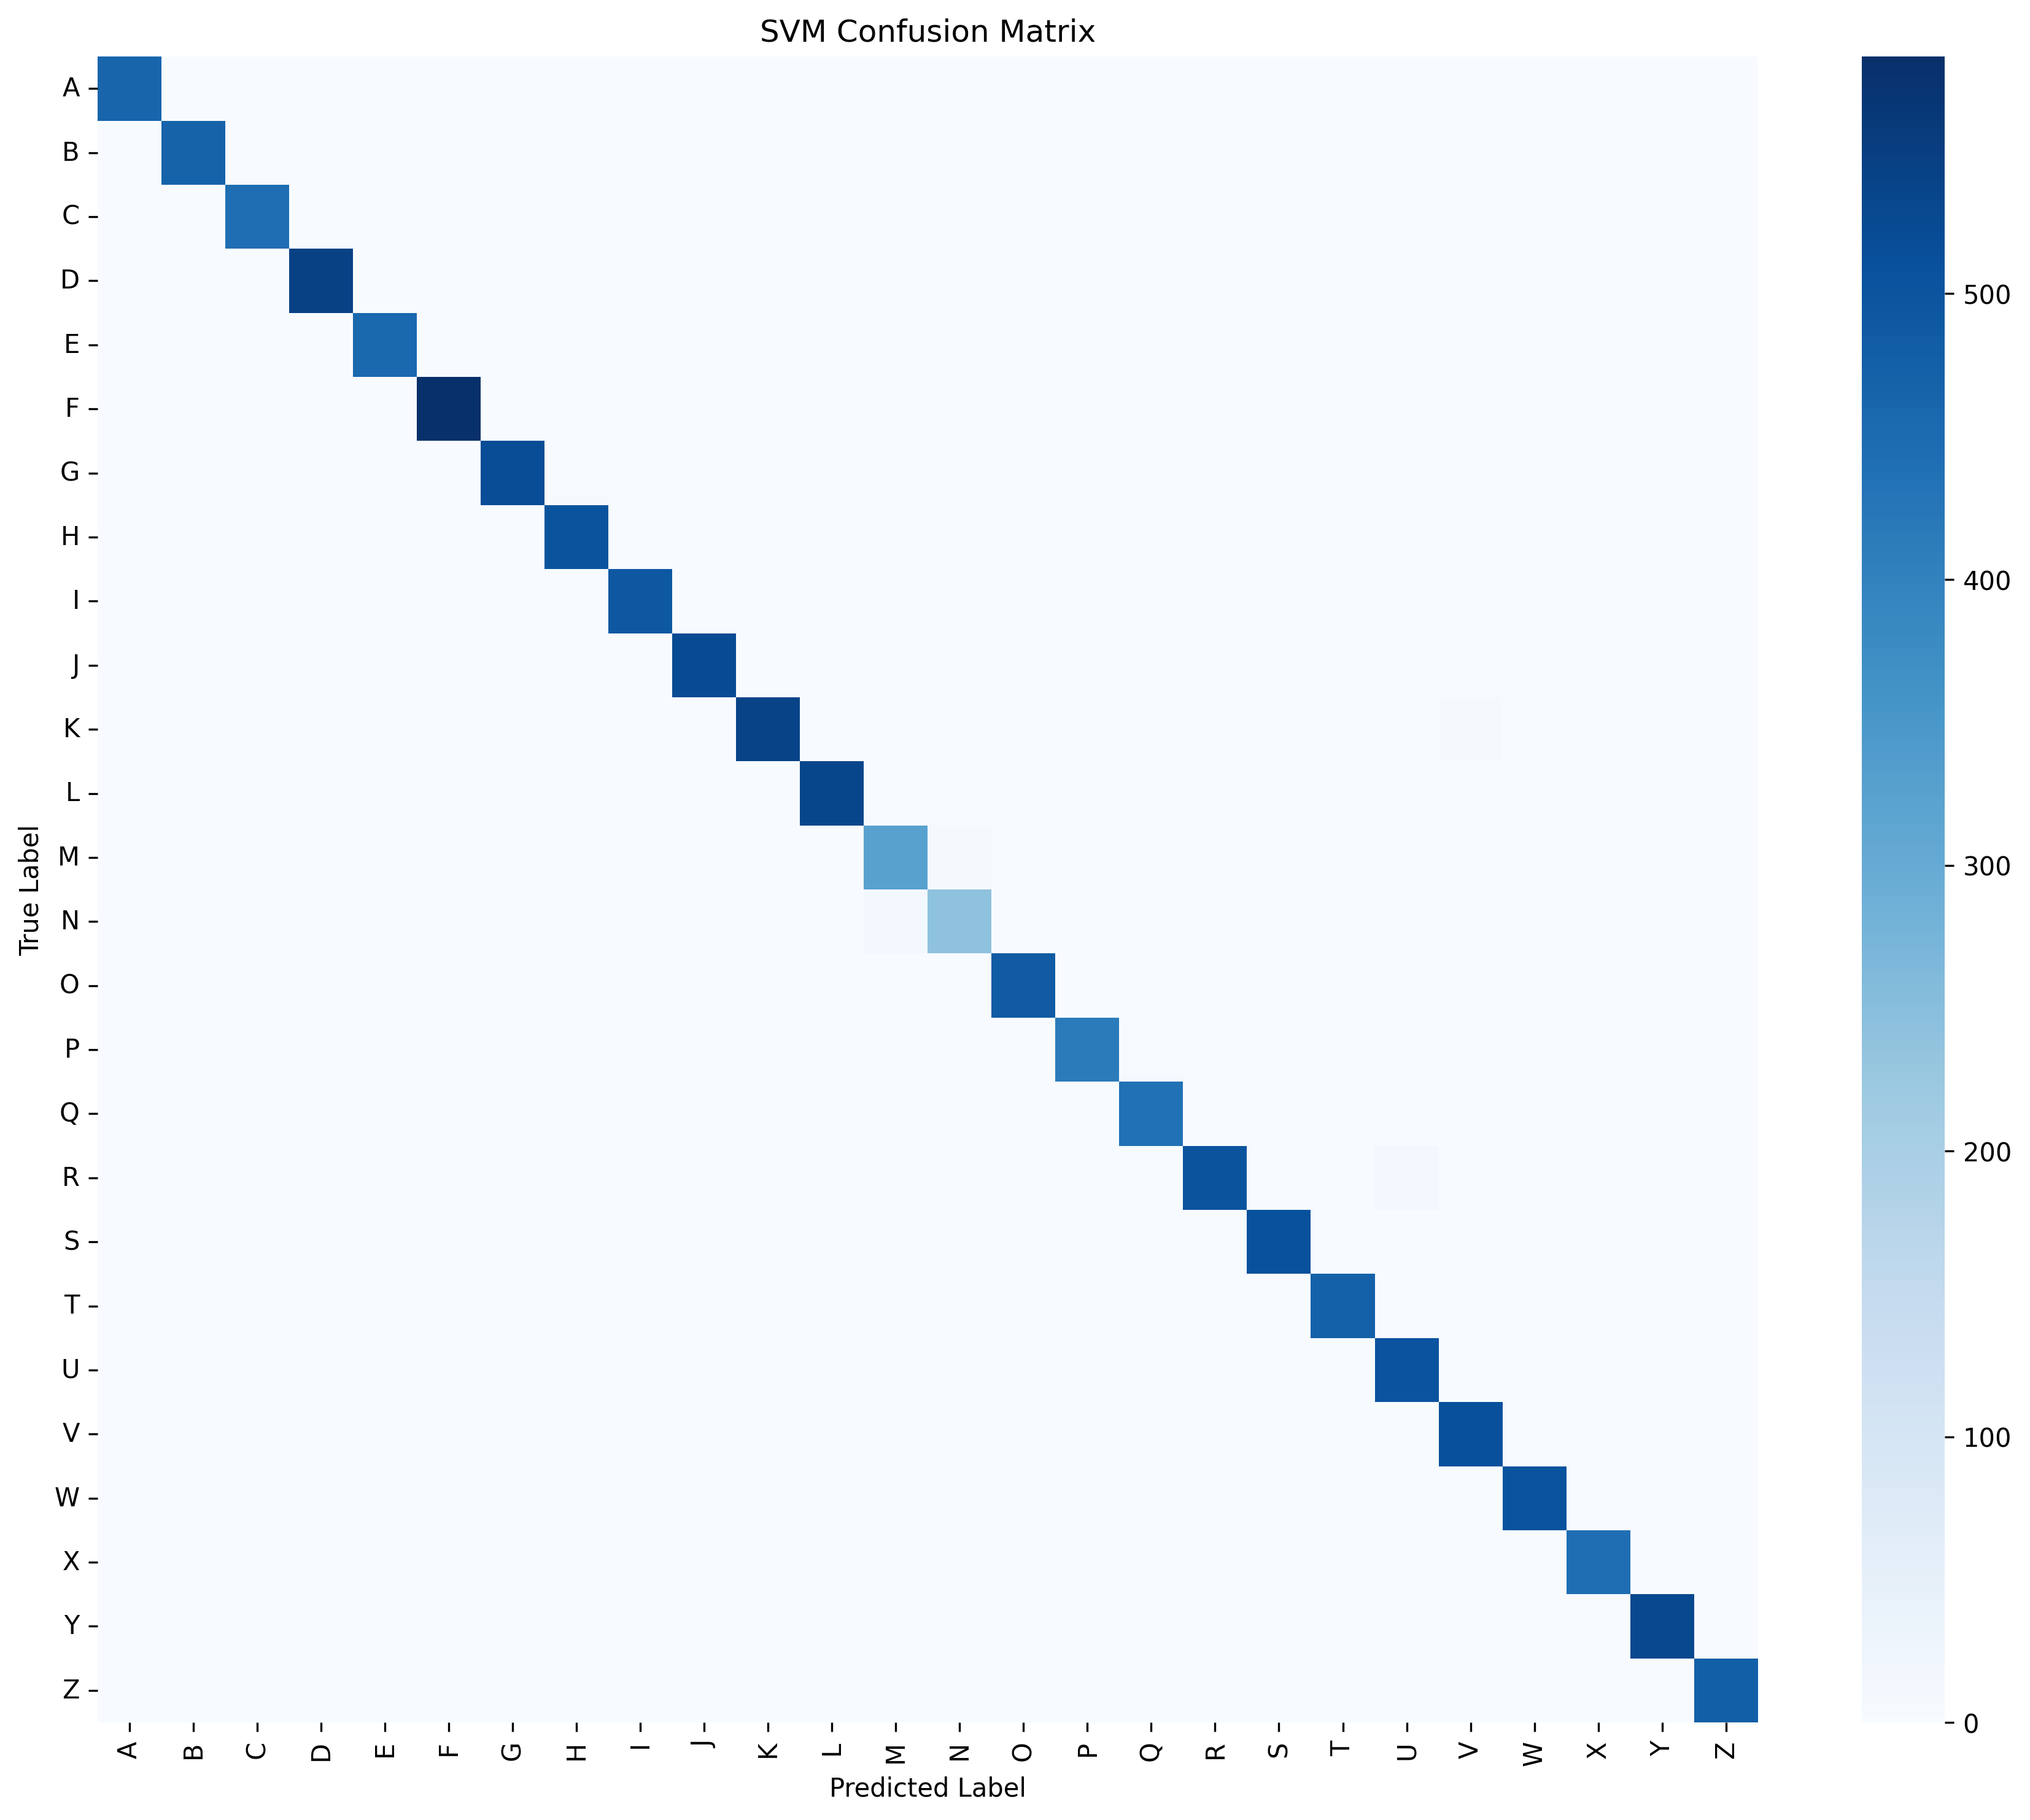
\includegraphics[width=0.75\linewidth]{images/SVM_confusion_matrix.png}
\end{figure}

Figure 1 shows a strong concentration of values along the diagonal, indicating that the majority of ASL alphabet gestures were correctly classified by the model. This demonstrates that the SVM classifier was highly effective in learning and distinguishing the spatial patterns derived from MediaPipe hand landmark coordinates. The high number of correct predictions across most classes confirms the reliability and robustness of the proposed approach for ASL gesture recognition.

Only minimal off-diagonal values were observed, suggesting that misclassifications occurred infrequently and were limited to a few visually similar hand gestures. These minor classification errors may be attributed to similarities in finger positioning and hand orientation between certain ASL letters, which can produce overlapping landmark patterns. Despite these challenges, the overall confusion matrix indicates that the SVM model maintained highly accurate and consistent predictions across the dataset.


\subsection{Feature Analysis and Importance of Hand Landmarks}

The extracted MediaPipe hand landmarks produced a structured 63-dimensional feature representation composed of the $(x, y, z)$ coordinates of 21 detected hand keypoints. These landmarks encoded the spatial arrangement of the wrist, finger joints, and fingertips, enabling the machine learning models to distinguish ASL alphabet gestures based on hand geometry rather than raw pixel information.

The high classification performance achieved by the SVM, Random Forest, and k-NN models indicates that the landmark features formed highly discriminative patterns within feature space. The SVM model achieved the highest overall accuracy of 98.8\%, suggesting that the extracted landmark coordinates provided sufficient spatial information for separating ASL classes with minimal overlap. Similarly, Random Forest and k-NN also achieved strong performance, indicating that the landmark representation effectively preserved gesture-specific structural characteristics.

The confusion matrix analysis further demonstrated the effectiveness of the extracted hand landmarks. Most predictions were concentrated along the diagonal of the confusion matrix, indicating that the landmark coordinates successfully captured the distinguishing spatial configurations of the ASL gestures. Misclassifications occurred only in a small number of visually similar letters, particularly among gestures such as M, N, R, U, and V. These classes involve subtle variations in finger positioning, overlap, and orientation, which can produce closely related landmark coordinate distributions.

The lower performance of Gaussian Naïve Bayes also highlighted the importance of spatial relationships among the landmark features. Unlike the other evaluated models, Naïve Bayes assumes feature independence, which is inconsistent with hand landmark data where finger and joint coordinates are strongly correlated. The significantly lower accuracy of Naïve Bayes suggests that the geometric dependencies between landmarks play a critical role in accurate ASL gesture recognition.
\section{Conclusion and Recommendations}

\subsection{Conclusion}
Among the evaluated models, the Support Vector Machine (SVM) achieved the highest overall performance, demonstrating superior classification capability compared to k-Nearest Neighbors (k-NN), Random Forest, and Naive Bayes. The SVM model obtained the highest accuracy and F1-score, indicating its effectiveness in learning discriminative patterns from the extracted image features and handling variations in hand gestures. The confusion matrix analysis further confirmed the reliability of the model, as most predictions were correctly classified with minimal misclassification across the ASL alphabet classes.

The results also showed that Random Forest and k-NN produced competitive performance, suggesting that these models are also capable of recognizing ASL gestures with high accuracy. In contrast, Naive Bayes exhibited significantly lower performance, indicating limitations in modeling the complex and non-linear relationships present in hand gesture image data.

Overall, the findings of the study demonstrate that machine learning techniques, particularly SVM, can effectively support the automated recognition of American Sign Language. The study highlights the potential of machine learning-based ASL recognition systems in improving accessibility and communication for individuals who rely on sign language.

\subsection{Recommendations}

Based on the findings of the study, several recommendations are proposed for future research and improvement of American Sign Language (ASL) recognition systems. Future studies may utilize larger and more diverse ASL datasets to improve the robustness and generalization capability of machine learning models across different hand shapes, lighting conditions, and backgrounds. Additional preprocessing and feature extraction techniques may also be explored to further enhance classification accuracy and minimize misclassification between visually similar gestures.

Moreover, future researchers may investigate the use of advanced deep learning architectures such as Convolutional Neural Networks (CNN), EfficientNet, ResNet, and Vision Transformers to compare their performance with traditional machine learning models. Since this study focused primarily on static ASL alphabet recognition, future work may also consider dynamic sign recognition involving motion-based gestures and continuous sign language translation to create more comprehensive communication systems.

The development of a real-time ASL recognition application using webcams, mobile devices, or embedded systems is also recommended to evaluate the practical applicability of the proposed approach in real-world environments. Furthermore, future studies may include additional evaluation metrics such as computational efficiency, inference time, and robustness under varying environmental conditions. Integrating ASL recognition systems with speech synthesis or text generation technologies may also further improve accessibility and communication support for deaf and hard-of-hearing individuals.

\section{Appendix}

\begin{table}[H]
\centering
\small
\renewcommand{\arraystretch}{1.2}
\setlength{\tabcolsep}{10pt}
\caption{SVM Performance on Test Set}
\begin{tabular}{|p{2cm}|cccc|}
\hline
\textbf{Label}& \textbf{Precision} & \textbf{Recall} & \textbf{F1-score} & \textbf{Support} \\
\hline
A & 1.00 & 1.00 & 1.00 & 465 \\
B & 0.99 & 1.00 & 1.00 & 469 \\
C & 0.99 & 1.00 & 1.00 & 445 \\
D & 0.99 & 0.99 & 0.99 & 550 \\
E & 1.00 & 0.99 & 0.99 & 461 \\
F & 1.00 & 0.99 & 1.00 & 586 \\
G & 1.00 & 0.99 & 1.00 & 521 \\
H & 0.98 & 0.99 & 0.99 & 506 \\
I & 0.99 & 1.00 & 0.99 & 494 \\
J & 1.00 & 0.99 & 0.99 & 530 \\
K & 0.99 & 0.98 & 0.99 & 551 \\
L & 1.00 & 1.00 & 1.00 & 537 \\
M & 0.94 & 0.96 & 0.95 & 337 \\
N & 0.96 & 0.93 & 0.95 & 258 \\
O & 0.99 & 1.00 & 0.99 & 486 \\
P & 1.00 & 0.98 & 0.99 & 424 \\
Q & 0.98 & 1.00 & 0.99 & 438 \\
R & 0.98 & 0.96 & 0.97 & 524 \\
S & 0.99 & 1.00 & 0.99 & 512 \\
T & 1.00 & 0.99 & 0.99 & 476 \\
U & 0.97 & 0.98 & 0.98 & 513 \\
V & 0.98 & 0.98 & 0.98 & 520 \\
W & 0.98 & 0.99 & 0.99 & 512 \\
X & 0.98 & 1.00 & 0.99 & 444 \\
Y & 1.00 & 1.00 & 1.00 & 532 \\
Z & 1.00 & 0.99 & 1.00 & 481 \\
\hline
\textbf{Accuracy} & \multicolumn{4}{|c|}{0.99} \\
\textbf{F1-Score} & \multicolumn{4}{|c|}{0.99}  \\
\hline
\end{tabular}
\end{table}


\begin{table}[H]
\centering
\small
\renewcommand{\arraystretch}{1.2}
\setlength{\tabcolsep}{10pt}
\caption{k-NN Performance on Test Set}
\begin{tabular}{|p{2cm}|cccc|}
\hline
\textbf{Label}& \textbf{Precision} & \textbf{Recall} & \textbf{F1-score} & \textbf{Support} \\
\hline
A & 0.98 & 0.99 & 0.99 & 465 \\
B & 1.00 & 1.00 & 1.00 & 469 \\
C & 0.98 & 0.99 & 0.99 & 445 \\
D & 0.99 & 0.99 & 0.99 & 550 \\
E & 0.98 & 0.99 & 0.99 & 461 \\
F & 0.99 & 1.00 & 1.00 & 586 \\
G & 0.99 & 0.99 & 0.99 & 521 \\
H & 0.98 & 0.98 & 0.98 & 506 \\
I & 1.00 & 0.99 & 0.99 & 494 \\
J & 1.00 & 0.98 & 0.99 & 530 \\
K & 0.97 & 0.98 & 0.97 & 551 \\
L & 0.99 & 1.00 & 0.99 & 537 \\
M & 0.95 & 0.94 & 0.94 & 337 \\
N & 0.94 & 0.92 & 0.93 & 258 \\
O & 0.99 & 0.99 & 0.99 & 486 \\
P & 0.98 & 0.98 & 0.98 & 424 \\
Q & 0.98 & 0.99 & 0.98 & 438 \\
R & 0.97 & 0.94 & 0.95 & 524 \\
S & 0.98 & 0.99 & 0.98 & 512 \\
T & 1.00 & 0.98 & 0.99 & 476 \\
U & 0.89 & 0.93 & 0.91 & 513 \\
V & 0.96 & 0.93 & 0.95 & 520 \\
W & 0.99 & 1.00 & 0.99 & 512 \\
X & 0.99 & 0.98 & 0.99 & 444 \\
Y & 1.00 & 1.00 & 1.00 & 532 \\
Z & 1.00 & 0.99 & 1.00 & 481 \\
\hline
\textbf{Accuracy} & \multicolumn{4}{|c|}{0.98} \\
\textbf{F1-Score} & \multicolumn{4}{|c|}{0.98}  \\
\hline
\end{tabular}
\end{table}


\begin{table}[H]
\centering
\small
\renewcommand{\arraystretch}{1.2}
\setlength{\tabcolsep}{10pt}
\caption{Naive Bayes Performance on Test Set}
\begin{tabular}{|p{2cm}|cccc|}
\hline
\textbf{Label}& \textbf{Precision} & \textbf{Recall} & \textbf{F1-score} & \textbf{Support} \\
\hline
A & 0.41 & 0.67 & 0.51 & 465 \\
B & 0.53 & 0.70 & 0.61 & 469 \\
C & 0.78 & 0.45 & 0.57 & 445 \\
D & 0.83 & 0.63 & 0.72 & 550 \\
E & 0.21 & 0.50 & 0.30 & 461 \\
F & 0.93 & 0.72 & 0.81 & 586 \\
G & 0.79 & 0.69 & 0.74 & 521 \\
H & 0.71 & 0.57 & 0.63 & 506 \\
I & 0.50 & 0.47 & 0.48 & 494 \\
J & 0.73 & 0.60 & 0.66 & 530 \\
K & 0.33 & 0.51 & 0.40 & 551 \\
L & 0.62 & 0.65 & 0.63 & 537 \\
M & 0.42 & 0.28 & 0.33 & 337 \\
N & 0.41 & 0.70 & 0.52 & 258 \\
O & 0.58 & 0.73 & 0.64 & 486 \\
P & 0.68 & 0.63 & 0.65 & 424 \\
Q & 0.75 & 0.63 & 0.68 & 438 \\
R & 0.36 & 0.34 & 0.35 & 524 \\
S & 0.26 & 0.30 & 0.28 & 512 \\
T & 0.71 & 0.38 & 0.49 & 476 \\
U & 0.18 & 0.04 & 0.06 & 513 \\
V & 0.35 & 0.62 & 0.45 & 520 \\
W & 0.60 & 0.26 & 0.37 & 512 \\
X & 0.44 & 0.24 & 0.31 & 444 \\
Y & 0.47 & 0.46 & 0.47 & 532 \\
Z & 0.60 & 0.49 & 0.54 & 481 \\
\hline
\textbf{Accuracy} & \multicolumn{4}{|c|}{0.51} \\
\textbf{F1-Score} & \multicolumn{4}{|c|}{0.51}  \\
\hline
\end{tabular}
\end{table}


\begin{table}[H]
\centering
\small
\renewcommand{\arraystretch}{1.2}
\setlength{\tabcolsep}{10pt}
\caption{Random Forest Performance on Test Set}
\begin{tabular}{|p{2cm}|cccc|}
\hline
\textbf{Label}& \textbf{Precision} & \textbf{Recall} & \textbf{F1-score} & \textbf{Support} \\
\hline
A & 0.99 & 0.99 & 0.99 & 465 \\
B & 0.99 & 1.00 & 0.99 & 469 \\
C & 0.99 & 1.00 & 0.99 & 445 \\
D & 0.99 & 0.99 & 0.99 & 550 \\
E & 0.98 & 0.99 & 0.99 & 461 \\
F & 0.99 & 1.00 & 0.99 & 586 \\
G & 0.99 & 0.99 & 0.99 & 521 \\
H & 0.99 & 0.98 & 0.98 & 506 \\
I & 1.00 & 1.00 & 1.00 & 494 \\
J & 0.99 & 0.98 & 0.99 & 530 \\
K & 0.99 & 0.99 & 0.99 & 551 \\
L & 1.00 & 0.99 & 0.99 & 537 \\
M & 0.95 & 0.96 & 0.96 & 337 \\
N & 0.96 & 0.93 & 0.94 & 258 \\
O & 0.98 & 0.99 & 0.98 & 486 \\
P & 0.99 & 0.99 & 0.99 & 424 \\
Q & 0.99 & 1.00 & 0.99 & 438 \\
R & 0.99 & 0.96 & 0.97 & 524 \\
S & 0.99 & 0.98 & 0.98 & 512 \\
T & 0.99 & 0.99 & 0.99 & 476 \\
U & 0.95 & 0.96 & 0.96 & 513 \\
V & 0.97 & 0.98 & 0.98 & 520 \\
W & 0.99 & 1.00 & 0.99 & 512 \\
X & 0.98 & 1.00 & 0.99 & 444 \\
Y & 1.00 & 1.00 & 1.00 & 532 \\
Z & 1.00 & 0.99 & 0.99 & 481 \\
\hline
\textbf{Accuracy} & \multicolumn{4}{|c|}{0.99} \\
\textbf{F1-Score} & \multicolumn{4}{|c|}{0.99}  \\
\hline
\end{tabular}
\end{table}



\begin{thebibliography}{99}

\bibitem{bakershenk1980}
Baker-Shenk, C., \& Cokely, D. (1980). \textit{American Sign Language: A Teacher's Resource Text on Grammar and Culture}. Gallaudet University Press, Washington, D.C.

\bibitem{adeyanju2021}
Adeyanju, I. A., Bello, O. O., \& Adegboye, M. A. (2021). Machine learning methods for sign language recognition: A critical review and analysis. \textit{Intelligent Systems with Applications, 12}, 200056. \\
https://doi.org/10.1016/j.iswa.2021.200056

\bibitem{bantupalli2018}
Bantupalli, K., \& Xie, Y. (2018). American sign language recognition using deep learning and computer vision. In \textit{Proceedings of the IEEE International Conference on Big Data} (pp. 4896--4899). IEEE. \\
https://doi.org/10.1109/BigData.2018.8622141

\bibitem{barczak2011}
Barczak, A. L. C., Reyes, N. H., Abastillas, M., Piccio, A., \& Susnjak, T. (2011). A new 2D static hand gesture colour image dataset for ASL gestures. \textit{Research Letters in the Information and Mathematical Sciences, 15}, 12--20.

\bibitem{hasan2012}
Hasan, M. M., \& Mishra, P. K. (2012). Hand gesture modeling and recognition using geometric features: A review. \textit{Canadian Journal on Image Processing and Computer Vision, 3}(1), 12--26.

\bibitem{isaacs2004}
Isaacs, J., \& Foo, S. (2004). Hand pose estimation for American Sign Language recognition. In \textit{Proceedings of the 36th Southeastern Symposium on System Theory} (pp. 132--136). IEEE. \\
https://doi.org/10.1109/SSST.2004.1295608

\bibitem{oz2011}
Oz, C., \& Leu, M. C. (2011). American Sign Language word recognition with a sensory glove using artificial neural networks. \textit{Engineering Applications of Artificial Intelligence, 24}(7), 1204--1213. \\
https://doi.org/10.1016/j.engappai.2011.03.015

\bibitem{pugeault2011}
Pugeault, N., \& Bowden, R. (2011). Spelling it out: Real-time ASL fingerspelling recognition. In \textit{Proceedings of the IEEE International Conference on Computer Vision Workshops} (pp. 1114--1119). IEEE. \\
https://doi.org/10.1109/ICCVW.2011.6130409

\bibitem{rish2001}
Rish, I. (2001). An empirical study of the Naive Bayes classifier. In \textit{IJCAI Workshop on Empirical Methods in Artificial Intelligence} (Vol. 3, No. 22, pp. 41--46).

\bibitem{who2021}
World Health Organization. (2021). \textit{World Report on Hearing}. WHO Press, Geneva, Switzerland. \\
https://www.who.int/publications/i/item/world-report-on-hearing

\bibitem{zhang2020}
Zhang, F., Bazarevsky, V., Vakunov, A., Tkachenka, A., Sung, G., Chang, C.-L., \& Grundmann, M. (2020). \textit{MediaPipe Hands: On-device real-time hand tracking}. arXiv preprint arXiv:2006.10214. \\
https://arxiv.org/abs/2006.10214

\end{thebibliography}
\end{document}